\documentclass{report}
\usepackage{fullpage}
\usepackage[margin=0.5in]{geometry}
\usepackage{hyperref}
\usepackage{amsfonts}
\usepackage{float}
\usepackage{graphicx}
\usepackage{caption}
\usepackage{subcaption}
\usepackage{color}
\renewcommand{\baselinestretch}{2}
\author{Steven Englehardt, Maciej Halber, Elena Sizikova}
\title{Understanding Collections of Images \\ \small{COS 521 Final Project Report}}
\begin{document}
\maketitle
\tableofcontents

\chapter{Introduction}
\section{Abstract}
This report explores a variety of image properties which make it possible to understand and explore collections of images. In particular, we look at how properties like color distribution, saturation, sharpness, and detail can be extracted and compared between images. To perform these task we usemethods such as Fast Fourier Transform (FFT) and Singular Value Decomposition (SVD). We seek to understand how the theoretical underpinnings of these two algorithms affect the way the images are formed in the first place. Ultimately, we provide a way of decomposing the image into mathematical notation (a descriptor) that differentiates well between a collection of images.

\section{Background Work}
{\color{red} I'll look at this section closer tmrw, definietly needs some expanding. Will add some color histogram stuff  -- Maciej}

There are many possible situations in which we would need to understand and compare image structure. For example, one might like to search for a location in which a photograph was taken, by looking at all the other available images, and finding the image closest to the search image. Alternatively, one may want to cluster images based on their content, and see what categories the image collection can be decomposed to. Both of these would be easy problems to solve, if the images were annotated with words: textual search is a well-solved problem. However, when the images are not labelled (this is known as unsupervised learning), and the image collection is extremely large, it is impractical to label the images by hand. For such problems, it is important to analyze image content automatically.

Existing methods of image search by analyzing content of the image include Google Goggles and Google Image Search, both are based on similar technology \cite{google_blog}, which checks for distinctive points, analyzes lines and textures and finally creates a mathematical model of the image. While the exact implementation is not available, Google Image Search does not provide clustering capabilities of analyzing existing input datasets. A more closer work is that of Oliva and Torralba \cite{gist_descriptor} which create a GIST descriptor (cite Freedmans work!!!), and use perceptual dimensions (naturalness, openness, roughness, expansion, ruggedness) to classify natural images, for example, pictures of coasts, mountains or cities. The authors work with a low dimensional representation of the scene which is collectively known as the \emph{Spatial Envelope}. The properties of the spatial envelope are estimated by means of Discrete Fourier Transform (DFT), Windowed Fourier transform (WFT), as well as spectral properties of the image are estimates (!!!! Expand). 

Having completed a graduate course in algorithms, our goal was to understand the results that were obtained by such a study, and specifically answer the question: why can we estimate proporties of the spatial envelope the way \cite{gist_descriptor} does? 


\chapter{Methods}
In this work, we focused on three directions to analyze the image structure, being color distributions, frequency distribution and geometrical structure. Color distribution is widely analyzed using color histograms, frequencies can be easily investigated using Fast Fourier Transform. For geometrical structure we have decided to explore the Singular Value Decomposition of the image in hope of discovering some useful properties ( see chapter \ref{sec:SVD} ). 

 
%   We first started with a collection of color images that were analyzed by the method of Color Histograms. We also analyzed the properties of the FFT method and the SVD method on the corresponding greyscale images. The resulting descriptors were then compared against each other and subsequently combined into a joint descriptor, that used the information from all three methods to describe images.

\section{Data}
%We tested the descriptors on two data-sets ?????
The dataset that we have used for exploring the image structure has been provided with work by Oliva and Torralba \cite{gist_descriptor}. The dataset contains images from 8 categories, {\color{red} Expand!}

\section{Implementation}

When factoring images using SVD or working with the FFT of an image, we chose to work in grayscale. The choice to do so was motivated by the desire to explore the physical meaning of the decomposition or transformation in the context of images. Though it is entirely possible to separate the red, green, and blue channels and work with each separately, it is difficult to determine whether relative differences in colors or deeper properties of the decomposition/transformation are leading to the observed descriptor performance. To do the conversion we used matlab's built-in \textit{rgb2gray} function, which removes hue and saturation information but preserves luminance. {\color{red} Above sentence is not exactly true - recovering luminance vs preserving color is a huge area of work, basically look up for integral images if interested. Will have to tweak the section a bit -- [Steve] - that sentence was lifted from the matlab documentation, see: \url{http://www.mathworks.com/help/images/ref/rgb2gray.html}, that is the extent of my knowledge, so feel free to update.}

\section{Color Analysis}
We began the exporation of image properties by considering the color distribution. In particular, the range of image colors that can be seen on a computer monitor are known as \emph{gamut}, see \cite{color_model_ref}. As we only considered computer images in .jpg and .png formats, we were mainly concerned with the models that represent the gamut. One of the most common such models is known as the RGB model, in which color at every pixel is a combination of three intensity values, of the Red, Green, and Blue colors.  
\begin{figure}[hbtp]
\centering
\caption{RGB Cube Model}
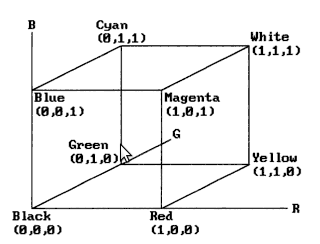
\includegraphics[scale=0.5]{graphics/rgb_cube.png}
\end{figure}

The Hue-Saturation-Value (HSV) Hexcone model is a fairly straightforward transformation from the RGB model, as shown in \ref{fig:hsv_visualisation}.
\begin{figure}[hbtp]
        \centering
        \begin{subfigure}[b]{0.3\textwidth}
                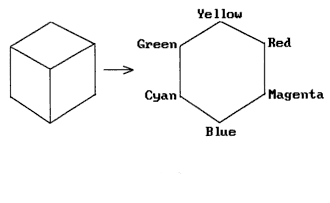
\includegraphics[width=\textwidth]{graphics/hsv_cube.png}
                \caption{The RGB cube viewed along Black-White diagonal}
                \label{fig:gull}
        \end{subfigure}%
        ~
         %add desired spacing between images, e. g. ~, \quad, \qquad etc.
          %(or a blank line to force the subfigure onto a new line)
        \begin{subfigure}[b]{0.3\textwidth}
                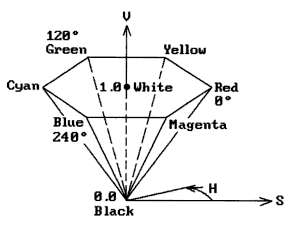
\includegraphics[width=\textwidth]{graphics/hsv_rescale1.png}
                \caption{Recoordination}
                \label{fig:mouse}
        \end{subfigure}
        ~
         %add desired spacing between images, e. g. ~, \quad, \qquad etc.
          %(or a blank line to force the subfigure onto a new line)
        \begin{subfigure}[b]{0.3\textwidth}
                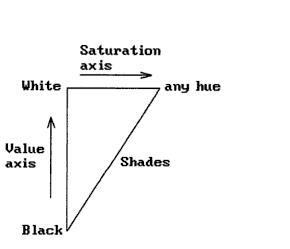
\includegraphics[width=\textwidth]{graphics/hsv_rescale2.png}
                \caption{Hue-Saturation Triangle}
                \label{fig:tiger}
        \end{subfigure}
        \caption{Transformation of the RGB cube to HSV color space}\label{fig:hsv_visualisation}
\end{figure}
In particular, the hue varies from $0^{\circ}$ to $360^{\circ}$, and represents the color. The hue and value are numbers in the range $[0,1]$ which represent how far is the hue from white and black, respectively. As noted further in \cite{color_model_ref}, this model is representative of how artists select colors. We therefore also used the HSV model in our analysis as a first comparison to the RGB model.

[LAB color model intro !!!!!!!!!]

{\color{red} We need to think about how much we want to talk to colors, especially when the performace between different color space descriptors is negligible. I would introduce the color spaces, and using them motivate the need for having simple parameters which allow for straightforward exploration }

\section{Fourier Transform} (????? what is the 2D FFT in terms of FFT {\color{red} FFT is just an algorithm for computing the fourier transform. We are less interested in the fact how it is able to perform the transform quickly and more in the properties of discrete fourier transform })
A $2$-dimensional, discrete Fourier Transform of an (grayscale) image is a transformation from the spatial domain to the frequency domain. In the spatial domain, an image is represented by function $f(x,y)$ on all relevant points $(x,y)$ in  $\mathbb{R}^2$. In the frequncy domain, the image is represented by a function $F(u,v)$ where $u$ and $v$ are frequency values. It follows that in the frequency decomposition, an image is represented by a matrix of complex values $F$, where $F(u,v)$ encodes the amplitude and the phase of the frequencies $u$ and $v$. Mathematically, the $2$-D Fourier Transform is defined as:
\begin{eqnarray}
F(u,v) = \int \int ^{\infty}_{-\infty} f(x,y)e^{-j2\pi (ux+vy)}dx dy
\end{eqnarray}
For $n$ points, we can compute the $1$-D DFT efficiently in $O(n\log{n})$ operations. The Matlab implemetation of the $2$-D FFT is extremely  fast, and we had no computational time issues with basing descriptors on these computations.

\subsection{Localization}
To understand the properties of the $2$-D Fourier Transform, we started by analyzying the $1$-D variant first. Consider the following functions, and their representations in the Fourier domain (\ref{fig:fft_localization}). A plot of $f(x)=\cos {x}$ is not very well localized in the spatial domain, that is the function could be said to be stretch along the x-axis. However it's representation in Fourier domain is extremly packed --- represented by a single peak. Conversely, $g(x)=\cos {50x}$ is well localized in the spatial domain, i.e. function can be thought of being squeezed along x-axis. In the Fourier domain, the same function is no longer localized - we observe the peaks to spread apart away from the zero value. This simple fact regarding the behavior of Fourier Transfrom suggested us a way of how to tackle images in the Fourier domain. Images containing a lot of high frequency periodicy ( buildings ) will have more contribution from these frequencies - by normalizing the image in Fourier domain we are able then to measure contribution from low frequencies. Again for a images with a lot of high frequency information we expect to observe less overall contribution after normalization.
\begin{figure}[h]
        \centering
        \begin{subfigure}[b]{0.2\textwidth}
                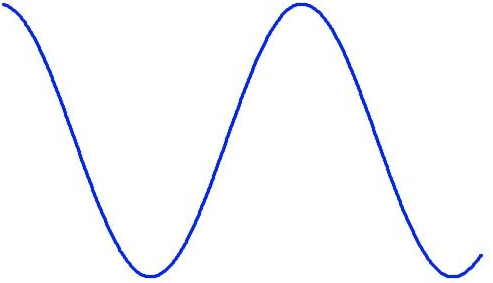
\includegraphics[width=\textwidth]{graphics/graph_fft_1.jpg}
                \caption{$f(x)=\cos{x}$}
                \label{fig:gull}
        \end{subfigure}%
        ~
         %add desired spacing between images, e. g. ~, \quad, \qquad etc.
          %(or a blank line to force the subfigure onto a new line)
        \begin{subfigure}[b]{0.2\textwidth}
                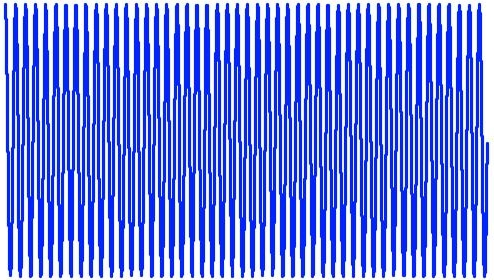
\includegraphics[width=\textwidth]{graphics/graph_fft_2.jpg}
                \caption{$g(x)=\cos{50x}$}
                \label{fig:tiger}
        \end{subfigure}
        
         %add desired spacing between images, e. g. ~, \quad, \qquad etc.
          %(or a blank line to force the subfigure onto a new line)
        \begin{subfigure}[b]{0.2\textwidth}
                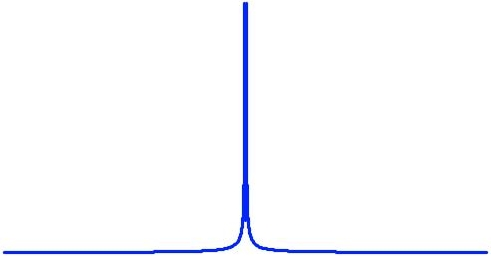
\includegraphics[width=\textwidth]{graphics/graph_fft_3.jpg}
                \caption{$F(f(x))$}
                \label{fig:mouse}
        \end{subfigure}
        ~
        \begin{subfigure}[b]{0.2\textwidth}
                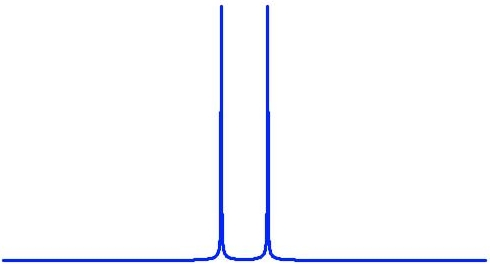
\includegraphics[width=\textwidth]{graphics/graph_fft_4.jpg}
                \caption{$F(g(x))$}
                \label{fig:mouse}
        \end{subfigure}
        \caption{Example of localization properties of different functions in the spatial and Fourier domains. Images localized in the spatial domain are not localized in the Fourier domain, and vice versa.}\label{fig:fft_localization}
\end{figure}

The given analysis yielded an easy descriptor, in which we sorted the images according the increasing contribution of low frequencies (alternatively, the decreasing contribution of high frequencies) \ref{fig:fft_low_freq_order} (!!!!!! Maciej, how exactly did you generate this?? Is this based on amplitude? {\color{red}Tried to scribble some explanation above, will need to go through it again}). The images should be read as one line that starts at top-left corner and ends in bottom-right. 

\begin{figure}[hbtp]
\centering
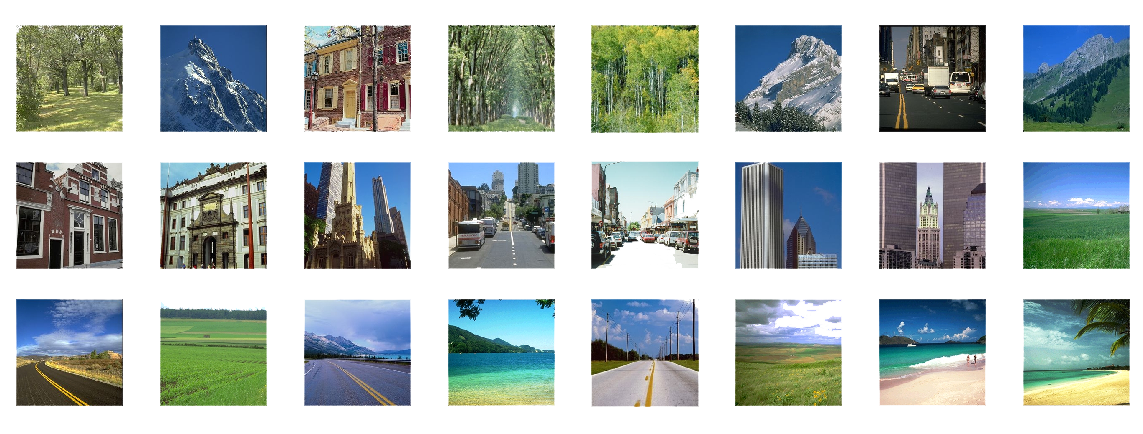
\includegraphics[scale=0.3]{graphics/FrequencyOrdered.png}
\caption{Ordering of a subset of the dataset by increasing contribution of low frequencies}
\label{fig:fft_low_freq_order}
\end{figure}
One can see that the images on the left side of the spectrum, with a lot of contribution from high frequencies and not so much from low frequencies have many small details: they show leaves, rock incisions on the mountain, and fine building facade. In comparison, the images at the right side of the spectrum are images of open country, roads, and beaches. These images are simple, in the sense that they have a dominant horizon line and not so much small detail. It follows that these images are described mostly by low frequencies, and not by high frequencies. Notice that this analysis discards a lot of information about the distribution of frequency contribution. We therefore proceeded into analyzing both phase and amplitude footprints of the image in greater detail.



\subsection{Amplitude and Phase Analysis}
Consider the decomposition of an image of a building in a city from the (???????????) GIST dataset into its frequency and amplitude footprints.
\begin{figure}[H]
        \centering
        \begin{subfigure}[b]{0.2\textwidth}
                
\includegraphics[width=\textwidth]{graphics/original.png}
                \caption{Original image}
                \label{fig:gull}
        \end{subfigure}%
        ~
         %add desired spacing between images, e. g. ~, \quad, \qquad etc.
          %(or a blank line to force the subfigure onto a new line)
        \begin{subfigure}[b]{0.2\textwidth}
                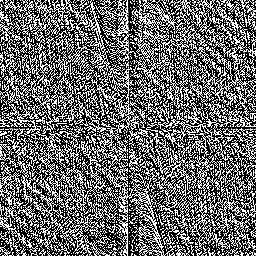
\includegraphics[width=\textwidth]{graphics/phase.png}
                \caption{Phase}
                \label{fig:mouse}
        \end{subfigure}
        ~
         %add desired spacing between images, e. g. ~, \quad, \qquad etc.
          %(or a blank line to force the subfigure onto a new line)
        \begin{subfigure}[b]{0.2\textwidth}
                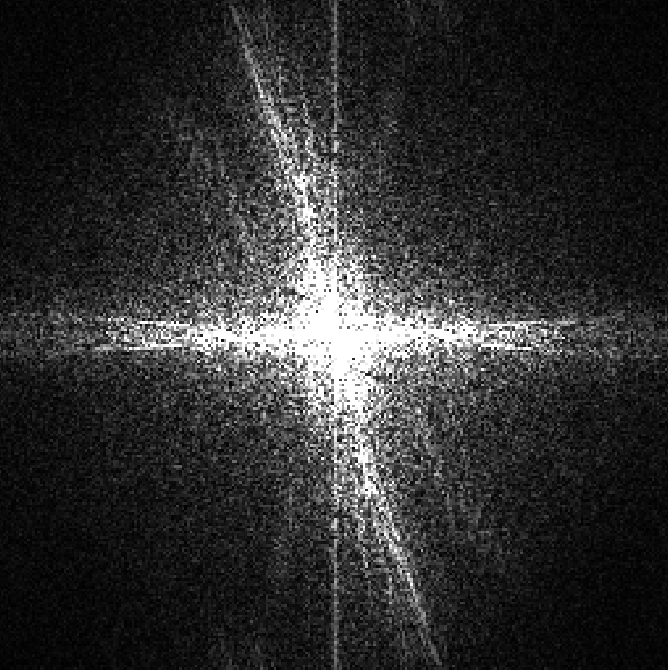
\includegraphics[width=\textwidth]{graphics/ampl.png}
                \caption{Amplitude}
                \label{fig:tiger}
        \end{subfigure}
        ~
        \begin{subfigure}[b]{0.2\textwidth}
                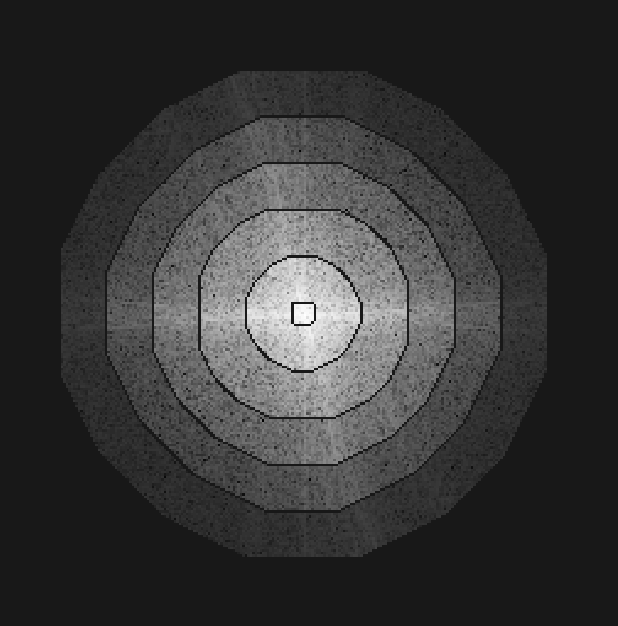
\includegraphics[width=\textwidth]{graphics/freq_bins.png}
                \caption{Frequency Bins}
                \label{fig:mouse}
        \end{subfigure}
        \caption{Example of localization properties of different functions in the spatial and Fourier domains. Images localized in the spatial domain are not localized in the Fourier domain, and vice versa.}\label{fig:fft_localization}
\end{figure}
As Oliva writes in \cite{gist_descriptor}, the phase image represents local properties of the image. It contains information relative to the form and the position of image components, while the amplitude talks about orientation, smoothness,
length and width of the contours in the given image. This can be further understood by taking the true phase values of the image, and setting all the amplitude values to $1$ (effectively taking out all amplitude variation and flattening the image), or taking true amplitude values and randomizing the phase:
\begin{figure}[H]
        \centering
        \begin{subfigure}[b]{0.2\textwidth}
                
\includegraphics[width=\textwidth]{graphics/original.png}
                \caption{Original image}
                \label{fig:gull}
        \end{subfigure}%
        ~
         %add desired spacing between images, e. g. ~, \quad, \qquad etc.
          %(or a blank line to force the subfigure onto a new line)
        \begin{subfigure}[b]{0.2\textwidth}
                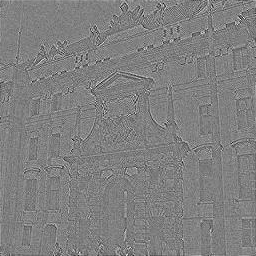
\includegraphics[width=\textwidth]{graphics/flat_power.jpg}
                \caption{Flat amplitude}
                \label{fig:mouse}
        \end{subfigure}
        ~
         %add desired spacing between images, e. g. ~, \quad, \qquad etc.
          %(or a blank line to force the subfigure onto a new line)
        \begin{subfigure}[b]{0.2\textwidth}
                
\includegraphics[width=\textwidth]{graphics/randomized_phase.jpg}
                \caption{Randomized phase}
                \label{fig:tiger}
        \end{subfigure}
        \caption{Analysis of Contributions of both Phase and Amplitude to an Image}\label{fig:fft_randomization}
\end{figure}
Note that a reconstructed image in which the amplitude information was not preserved retains the information about the edges and outlines in the original image. Conversely, the amplitude-preserved image is meaningless to out eyes: it shows the distribution and concentration of color. 




\section{Singular Value Decomposition}
\label{sec:SVD}
A deeper understanding of Singular Value Decomposition (SVD) in the context of images allows the creation of a descriptor that captures overall image complexity in a relatively small descriptor length. SVD is a factorization of any real or complex 2-dimensional matrix. Since images will always be represented by real matrices, we ignore the complex case in our analysis. 

Consider an $m \times n$ matrix $A$. The singular values of $A$  correspond to the non-zero square roots of the eigenvalues from $AA^T$ and $A^TA$. The matrix $AA^T$ is spanned by the row space of A, and the matrix $A^TA$ is spanned by the column space of $A$ \cite{using_svd}. The row space and column space being the set of all linear combinations of row vectors and column vectors of $A$, respectively.

SVD conveniently decomposes $A$, separating out singular values, row space eigenvectors, and column space eigenvectors into three different matrices. The SVD of $A$ is defined as:
$$A_{\scriptscriptstyle m \times n} = U_{\scriptscriptstyle m \times m}S_{\scriptscriptstyle m \times n}V_{\scriptscriptstyle n \times n}^T$$
where $S$ is a diagonal $m \times n$ matrix with the singular values of $A$ on the main diagonal (in decreasing order). The columns of $U$ are the eigenvectors of $AA^T$ and the columns of $V$ are the eigenvectors of $A^TA$ \cite{using_svd}. $U$ and $V$ are known as the left and right singular vectors of $A$, respectively.

The rank of a matrix is informally defined as a measure of the "nondegenerateness" of system of linear equations encoded by that matrix, or more formally is equal to the size of the row space or column space of the matrix. Linearly independent singular vectors correspond to non-degenerate singular values.  The rank of a matrix is thus equal to the number of non-degenerate singular values of the matrix, and is also equal to the number of linearly independent vectors in $U$ or in $V$. If all singular values are non-degenerate, $A$ is a full rank matrix and the SVD of $A$ is unique.

\subsection{SVD and Compression}
It is useful to think of each singular value in $S$ as scaling the row and column singular vectors from $U$ and $V$ to generate an 'eigenimage' \cite{svd_image_coding}, or the contribution of that specific singular value to the overall image. This construction is what enables image compression through a low-rank matrix approximation. Let $\tilde{A}$ represent the $k$-approximation of $A$, where $rank(\tilde{A}) = k$. Thus:
$$\tilde{A} = U(:,1:k)\tilde{S}V(:,1:k)^T$$

\begin{figure}[H]
        \centering
        \begin{subfigure}[b]{0.4\textwidth}
                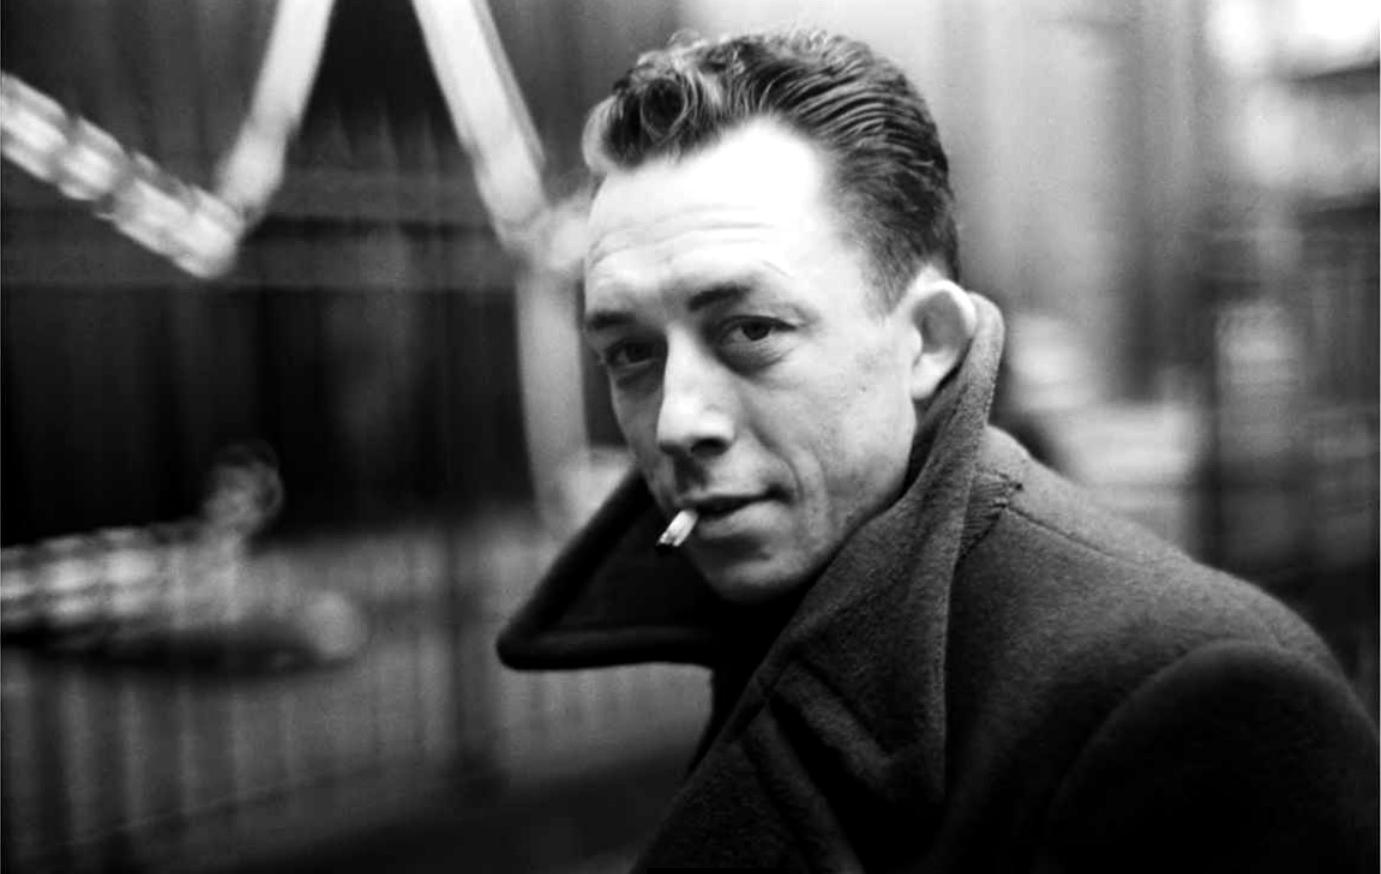
\includegraphics[width=\textwidth]{graphics/guy.jpg}
                \caption{Original image}
        \end{subfigure}
        \begin{subfigure}[b]{0.4\textwidth}
                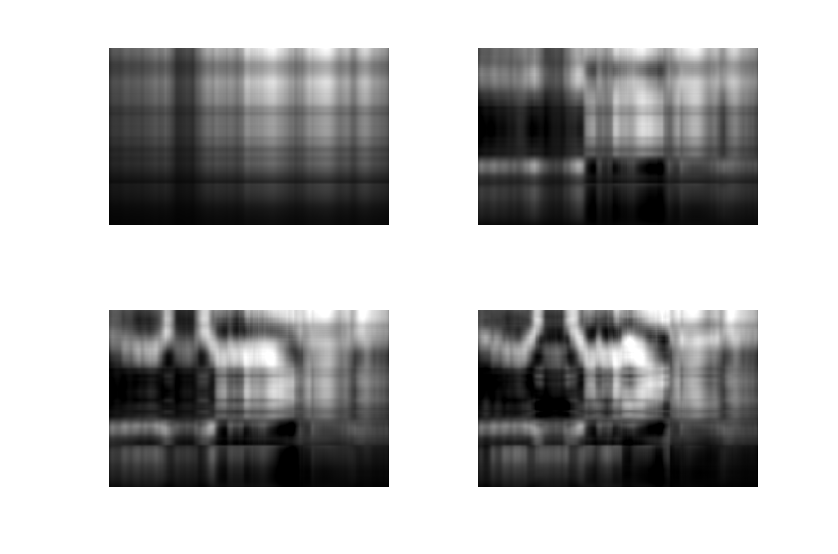
\includegraphics[width=\textwidth]{graphics/guyTopCompressions.png}
                \caption{Rank 1 to 4 from top left to bottom right}
        \end{subfigure}
        \caption{Rank k-approximations of an image using SVD}\label{fig:svd_compression}
\end{figure}

The performance of SVD in image compression shows that there is a significant amount of visual information in low rank approximations of images. Our desire is to capture this low rank information in a concise descriptor for use in image retrieval. An examination of both the singular values and the singular vectors follows.

\subsection{Singular Values}

Image retrieval using all singular values of a matrix has been shown to perform better than a simple distance metric, such as the Mahalanobis distance, Manhattan distance, or Euclidean distance \cite{svd_image_retrieval}. Several factors contribute to this performance, but relate to the fact that the distribution of singular values in $S$ is connected to the rank of $A$, the image matrix. 

The alignment of an images' strongest color contours to either the horizontal or vertical axis allow it to be fully captured in the left or right singular vectors of an image and thus requires few singular values. The means the image's matrix representation is of lower rank and thus loses less information by ignoring the smallest singular values. In an extreme example, the three images in Figure \ref{fig:rank1_images} can be fully represented using only the top singular value since they are all rank 1 matrices.

\begin{figure}[H]
        \centering
        \begin{subfigure}[b]{0.2\textwidth}
                
\includegraphics[width=\textwidth]{graphics/horizontalGrad.png}
                \caption{$S(1,1) = 37726$}
        \end{subfigure}
        ~~~
        \begin{subfigure}[b]{0.2\textwidth}
        		
\includegraphics[width=\textwidth]{graphics/smallVertical.png}
        		\caption{$S(1,1) = 46041$}
        \end{subfigure}
        ~~~
        \begin{subfigure}[b]{0.2\textwidth}
                
\includegraphics[width=\textwidth]{graphics/smallHorizontal.png}
                \caption{$S(1,1) = 46041$}
        \end{subfigure}
        \caption{Rank 1 images and their top singular value}
        \label{fig:rank1_images}
\end{figure}

On the opposite end of the spectrum, consider the randomly generated images in Figure \ref{fig:rand_images}. These three images are full rank and require all 256 singular values for a full reconstruction. The plot of the singular values from these images reveals that the range of intensity in the image directly correlates to the magnitude of the singular values needed, but has no correlation to the number of values needed.

\begin{figure}[H]
        \centering
        \begin{subfigure}[b]{0.2\textwidth}
                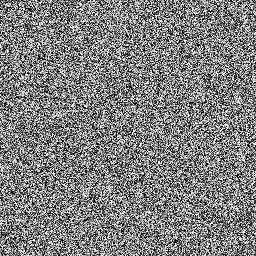
\includegraphics[width=\textwidth]{graphics/randomFullSpace.png}
                \caption{Full: $0-255$}
        \end{subfigure}
        ~~~
        \begin{subfigure}[b]{0.2\textwidth}
        		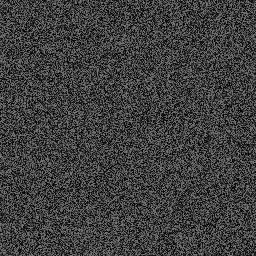
\includegraphics[width=\textwidth]{graphics/randomBottomHalfSpace.png}
        		\caption{Half: $0-127$}
        \end{subfigure}
        ~~~
        \begin{subfigure}[b]{0.2\textwidth}
                
\includegraphics[width=\textwidth]{graphics/randomBottomQuarterSpace.png}
                \caption{Quarter: $0-63$}
        \end{subfigure}

        \begin{subfigure}[b]{0.6\textwidth}
                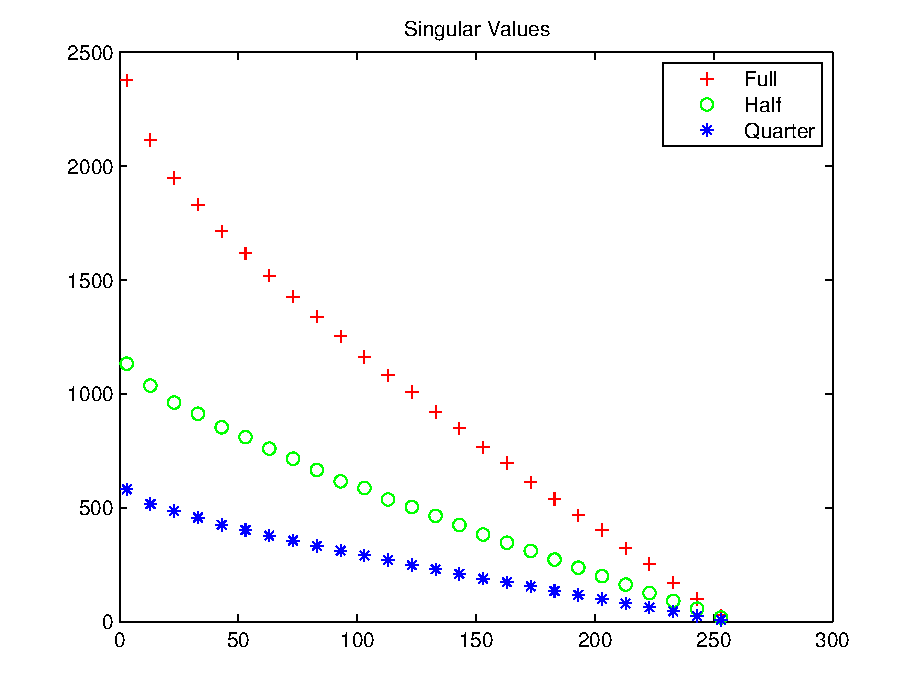
\includegraphics[width=\textwidth]{graphics/singular_values_color_space.pdf}
                \caption{Plot of singular values (1st value omitted for scaling)}
        \end{subfigure}
        \caption{(a-c): Random images with given intensity range (d): Singular values of (a-c)}
        \label{fig:rand_images}
\end{figure}

Figure \ref{fig:rank1_images} shows very simple rank 1 images that only require the 1st singular value, whereas Figure \ref{fig:rand_images} shows that full rank images requires all singular values. To get a better understanding of the required number of singular values we look at what happens when there is symmetry in the image. Figure \ref{fig:rand_symmetry} shows the plot of singular values from several random images which span the full intensity range from $0-255$, but have symmetry in various directions. In all images, the symmetry is about a central axis, so it covers half of the image.

\begin{figure}[H]
        \centering
        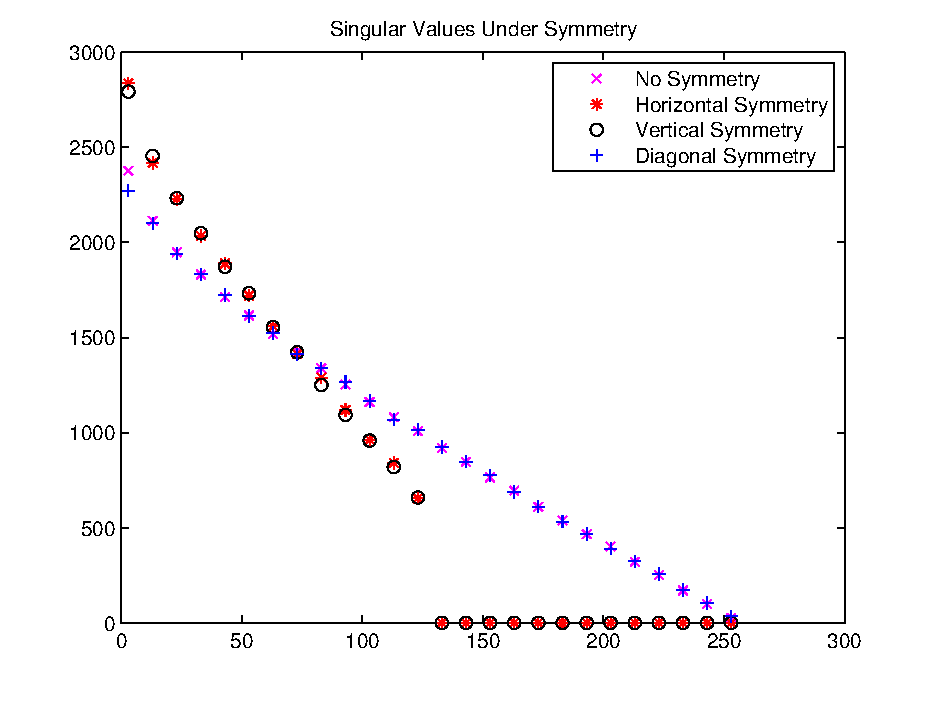
\includegraphics[width=0.6\textwidth]{graphics/singular_values_symmetry.pdf}
        \caption{Plot of singular values under symmetry (1st value omitted for scaling)}
        \label{fig:rand_symmetry}
\end{figure}

Figure \ref{fig:rand_symmetry} shows that the amount of symmetry within an image can greatly reduce the number of singular values required for reconstruction (in this case by half, since half of the image was repeated). However, this also shows a major issue with directly using the output of SVD for an image descriptor. An image which has symmetry off-axis at a $45^\circ$ angle will still have linearly independent vectors in $U$ and $V$ as the image is still full rank. Despite the fact that half of the image is repeated, the distribution of singular values is nearly identical to the image with no symmetry. It should be noted that $45^\circ$ is chosen because it represents the worst-case off-axis example. Angles above and below will experience some level of symmetry in either the horizontal or vertical direction.

\chapter{Analysis}

[Steve] I suppose that here we should give a brief summary of k-means clustering and multidimensional scaling, and then show the results of the descriptor (with and without windowing) and an analysis of that? I was planning to investigate the properties of SVD and show some basic performance results in the SVD section....but that presents the problem that I evaluate my results with k-means and k-means won't be introduced yet..

E: I think we can introduce K-means, embedding, search by query, and any other similar things we used to test descriptors with in the Methods section, all under one section, say testing framework?


\chapter{Suggestions for Further Work}
%\subsection{Your Subsection title here}
%\subsubsection{Your subsubsection title here}
%\paragraph{Your paragraph title here}
Just some quick ideas - our exploration assumed that each property is indepenend which is obviously not true, and it would be interesting to look at similarities/ collerations between SVD and FT. 
Our exploration was purely based on properties of algorithms and visual exploration using MDS and k-nearest neighbour searches. Our performance for retrival is not really measured other that providing visual examples - some improvements on this front would be nice.
Images are extremly high dimensional space, and our analysis might not be entirely revealing - using some machine learning techinques (vide Zeyu and Shuran ) could help us to learn some more about mentioned dimensionality independence etc.

\begin{thebibliography}{6}

\bibitem{google_blog}
  Johanna Wright,
  \emph{Search by Text, Voice, or Image}.
  Inside Search: Official Google Search Blog,
  2011.
  
\bibitem{gist_descriptor}
  Aude Oliva, Antonio Torralba,
  \emph{	Modeling the Shape of the Scene: a Holistic Representation of the Spatial Envelope}.
  International Journal of Computer Vision, 
  Vol. 42(3): 145-175, 
  2001.

\bibitem{using_svd}
  Ientilucci, Emmett J,
  \emph{Using the singular value decomposition}. 
  Chester F. Carlson Center for Imaging Science,
  Rochester Institute of Technology,
  2003.

\bibitem{svd_image_coding}
  Andrews, Harry C. and Patterson, C., III,
  \emph{ Singular Value Decomposition (SVD) Image Coding}.
  IEEE Transactions on Communications,
  Vol. 24(4): 425-432,
  1976.

\bibitem{svd_image_retrieval}
  Jie-xian Zeng; Dong-ge Bi; Xiang Fu,
  \emph{A Matching Method Based on SVD for Image Retrieval}.
  Measuring Technology and Mechatronics Automation, 2009. ICMTMA '09. International Conference on, 
  Vol. 1: 396-398, 
  11-12 April 2009
  
\bibitem{color_model_ref}
  Agoston, Max K.
  \emph{Computer Graphics and Geometric Modelling: Mathematics}.
  Springer; 2005 edition,
  ISBN:1852338172

\end{thebibliography}

\end{document}

